\chapter{Database Design}
\section{Entities, Attributes and Relationships}
The database, called data, will have eight tables, books, borrowed\_cars, cars, categories, engine\_types, system\_settings, transmission\_types and users. Each will hold information about either the cars and bookings. The two
tables will be linked through a foreign key. The  table has the following fields:\\
\begin{figure}[H]
\centering
\caption{Car Rental table}
\includegraphics[scale=.9]{./Blank Diagram}
\\[0.2in]
\label{fig:Car Rental}
\end{figure}


\section{Identify Major entities, attributes and relationships}
\begin{itemize}
\item Login page to give access to priviledged Admin.
\item Adding car details details by the Admin.
\item Changing the id and password of the staffs.
which stores the details of transaction.
\item Admin can check all details  and modify them.
\item Admin can delete the entities in the tables.
\item Easy  search facilities to get the reqiured information.
\end{itemize}
\section{ER Schema}
\begin{figure}[H]
\centering
\caption{Entity Relationship Diagram}
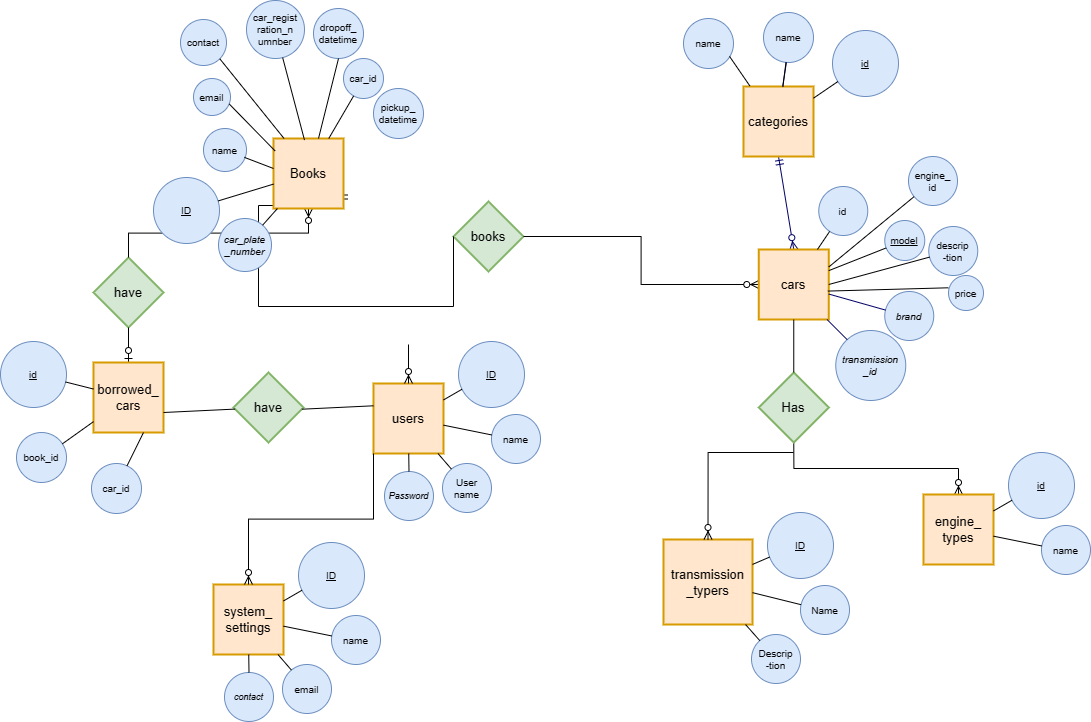
\includegraphics[width=\textwidth,height=\textheight,keepaspectratio]{./ER.png}
\\[0.2in]
\label{fig:Entitiy Relationship Diagram}
\end{figure}

\pagebreak
\thispagestyle{fancy}

\section{Schema Diagram}
\begin{figure}[H]
\centering
\caption{Relational Schema}
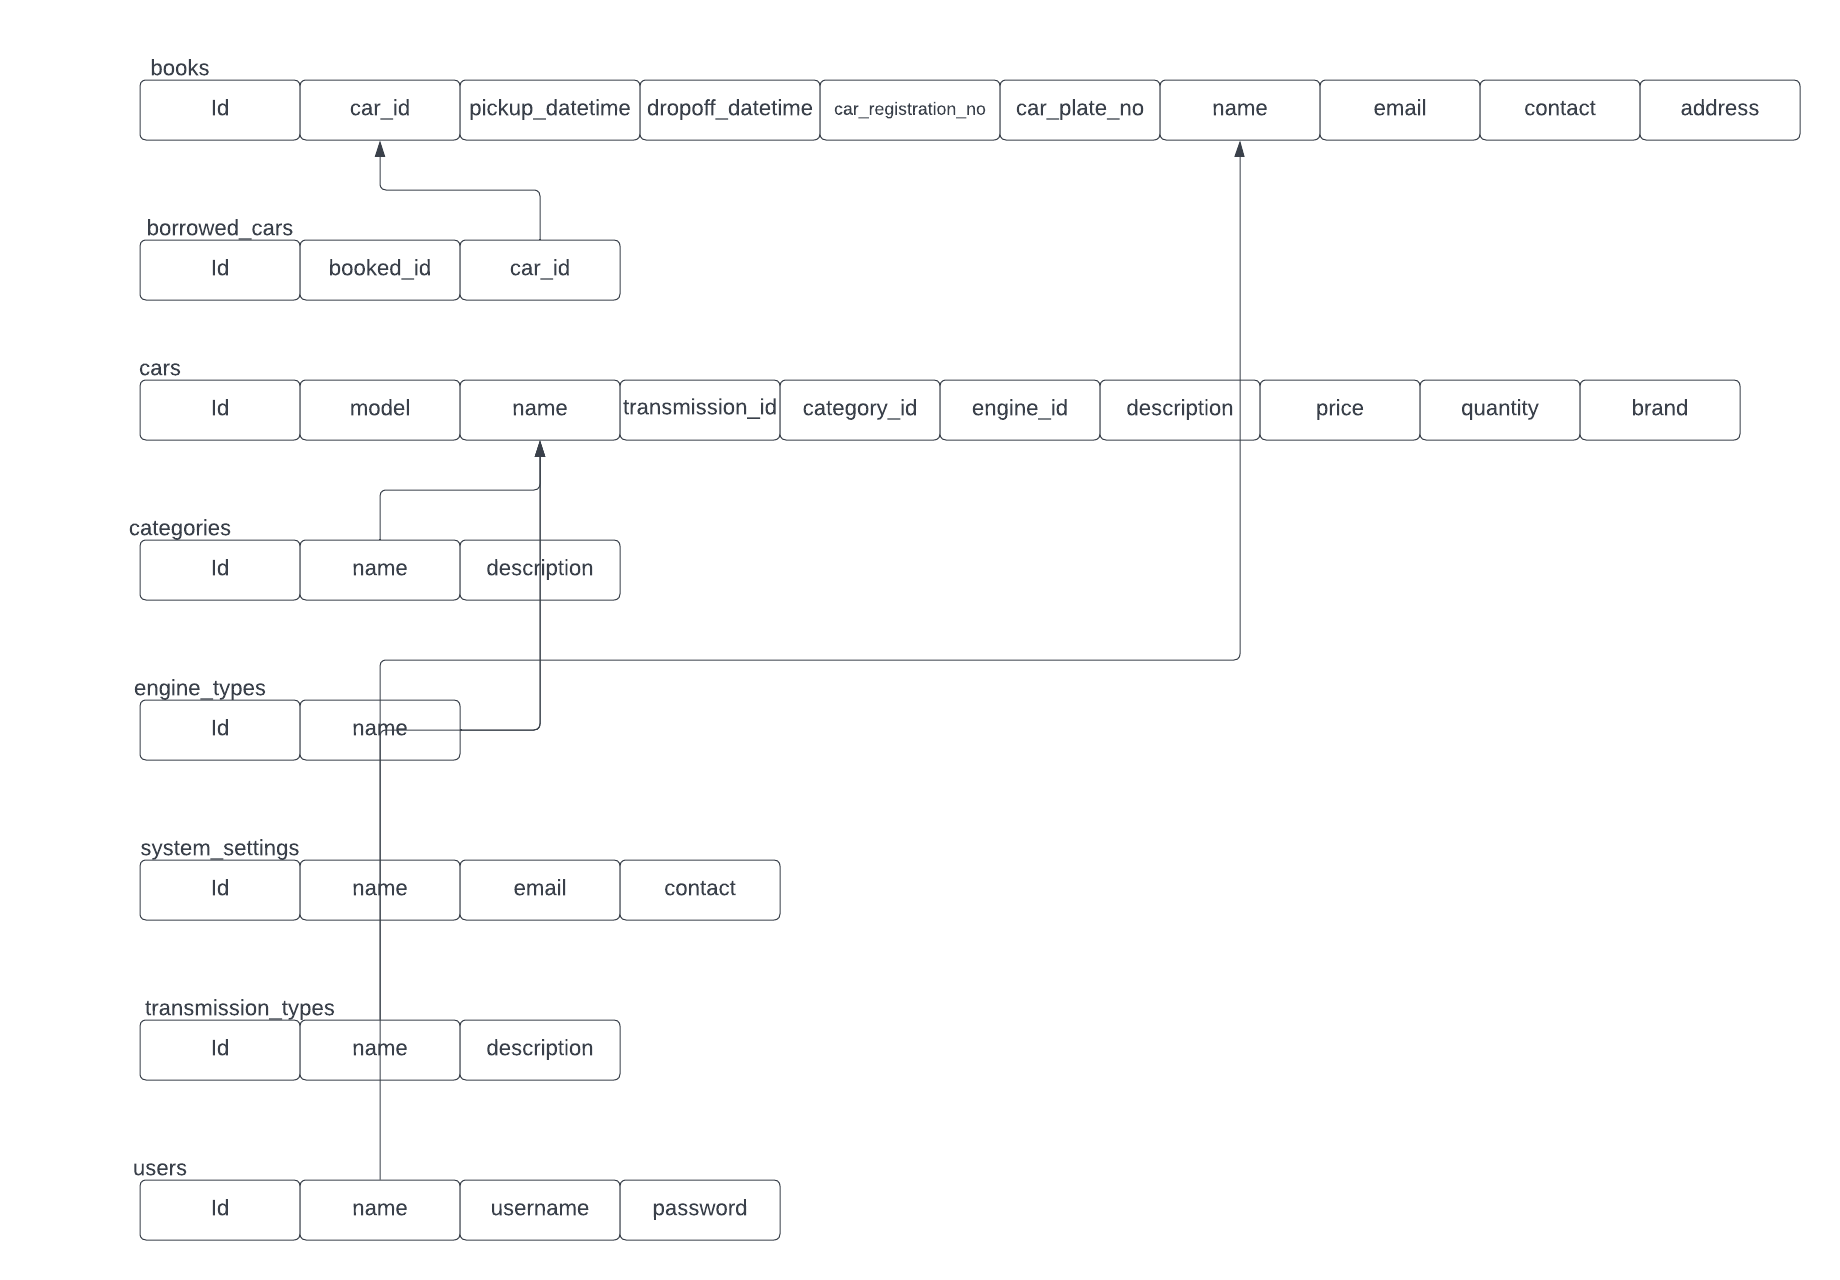
\includegraphics[scale=.65]{./Schema.png}
\\[0.2in]
\label{fig:Relational Schema}
\end{figure}

\thispagestyle{fancy}
